%----------------------------------------------------------
\def\notedate{2022.09.29}
\def\currentauthor{Василян А.Р. (РК6-73Б)}
%----------------------------------------------------------
\notestatement{rndhpcgui}{Программный инструментарий для создания подсистем ввода данных при разработке систем инженерного анализа}

%---------------------------------------------------------

Была изучена статья <<Программный инструментарий для создания подсистем ввода данных при разработке систем инженерного анализа>>. Из статьи были учтены основные определения, программный инструментарий. Автоматическое построение GUI -- построение графических форм ввода исходных данных для прикладной программы без участия человека с использованием программы-генератора GUI и файла исходных данных в специальном формате; Метаданные -- список входных параметров и их текущие значения в рамках выполнения прикладной программой вычислительной задачи.

На рисунке~\ref{rndhpcgui.2022.09.29.diagram} представлена диаграмма потока данных при построении и эксплуатации GUI на основе созданного программного инструментария и формата aINI. Описание некоторых процедур в схеме:
\begin{enumerate} [start=0]
	\item Процедура создания и редактирования списка входных данных осуществляется вручную с использованием доступных текстовых редакторов в формате aINI.
	\item Чтение aINI-файла осуществляется aINI-парсером, обеспечивающим синтаксический разбор конструкций aINI-файла, включая типы каждого параметра, и формирование aINI-объекта.
	\item Построение GUI осуществляется с помощью платформозависимого GUI-генератора, на вход которого подается aINI-объект во время выполнения прикладной программы, использующей соответствующий aINI-файл в качестве входных данных.
	\item Автоматическое обновление aINI-файла согласно внесенным пользователем изменениям в значения входных параметров в экранной форме. 
	\item Процедура ввода данных включает изменение текущих значений входных параметров и осуществляется в сформированной экранной форме. Количество и типы входных параметров при этом не изменяются.
	\item Создание объекта класса AnyMap, содержащего все входные параметры и их текущие значения (метаданные), осуществляется для возможности дальнейшей передачи на вход функциям обработки данных или для возможности передачи по сети на удаленный высокопроизводительный узел с целью проведения расчета на нем.
	\item Обновление объекта исходных данных класса AnyMap осуществляется после изменения значений в экранных формах.
	\item Непосредственная обработка объекта исходных данных класса AnyMap.
\end{enumerate}

\begin{figure}[!ht]
  \centering
  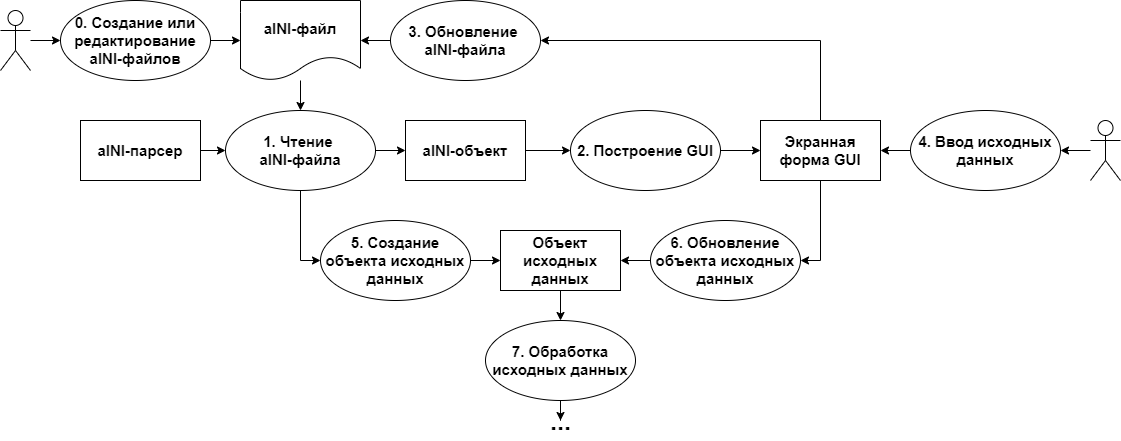
\includegraphics[scale=0.8]{ResearchNotes/rndhpc_int_gui_2022_09_29/diagram.png}
  \caption{Диаграмма потока данных при построении и эксплуатации GUI на основе созданного программного инструментария и формата aINI}
  \label{rndhpcgui.2022.09.29.diagram}
\end{figure}

После изучения статьи в качестве языка определения входных данных был выбран aINI, так как подготовка входных данных доступна для неподготовленного специалиста, не владеющего навыками программирования, в том числе для специалистов, представляющих заказчика разрабатываемой прикладной программы. Формат основан на известном языке INI.

Нотация Бэкуса-Наура. Форма Бэкуса -- Наура (сокр. БНФ, Бэкуса -- Наура форма) -- формальная система описания синтаксиса, в которой одни синтаксические категории последовательно определяются через другие категории. БНФ используется для описания контекстно-свободных формальных грамматик, обычно используется для описания синтаксиса языков программирования, форматов документов, наборов инструкций и протоколов связи. Применяются везде, где необходимо точное описание синтаксиса.

Терминал или терминальный символ -- объект, непосредственно присутствующий в словах языка, соответствующего грамматике, и имеющий конкретное, неизменяемое значение. Нетерминал или нетерминальный символ -- объект, обозначающий какую-либо сущность языка (например: формула, арифметическое выражение, команда) и не имеющий конкретного символьного значения. БНФ-конструкция определяет конечное число нетерминалов и определяет правила замены символа на какую-то последовательность терминалов и символов. За процессом построения цепочек букв можно проследить. Изначально имеется только один символ. Затем этот символ заменяется некоторой последовательностью букв и символов, согласно одному из описанных правил. Затем процесс повторяется (на каждом шаге один из символов заменяется на последовательность, согласно правилу).
%----------------------------------------------------------
% Атрибуты задачи
\noteattributes{}
%----------------------------------------------------------

